\subsection{Implementation}
%In our implementation, we are interesting in the following use case.

% \emph{Alice has an account with OpenStack Swift. She has an object `data.json' in a Swift container. She likes to share this object with her colleagues Bob and Charlie so that they can only see selective content of 'data.json' that she has authorized  them.}

%In the rest of this section, we specify required changes in Swift.




\subsubsection{Changes in Swift Object Server}

 We have extended  the logic of Swift Object Server. In the existing implementation, when a request comes for downloading of an object, Object Server checks the ACL and if the object is allowed by ACL, the Object Server reads the object from the disk and pass the whole content to the requester through Proxy-server.

\begin{figure}
  \centering
    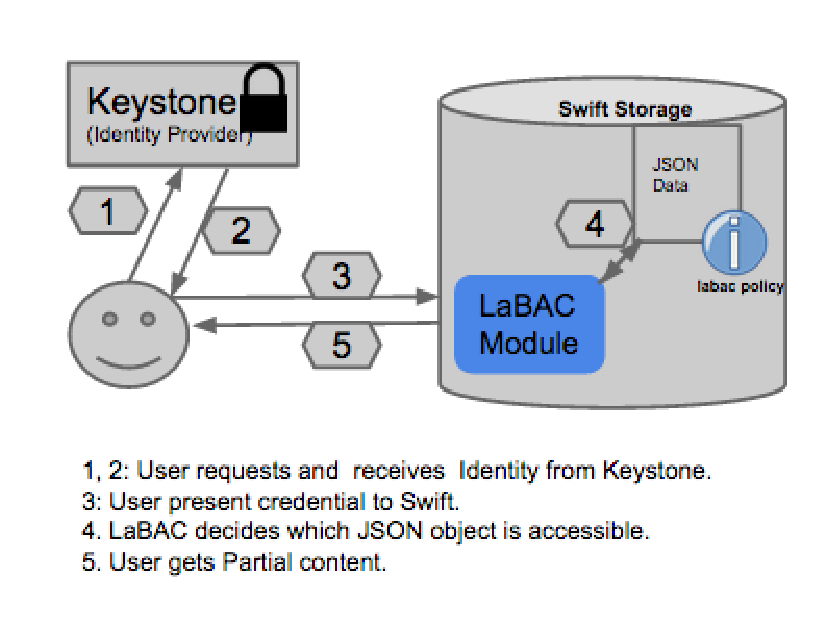
\includegraphics[width=0.5\textwidth]{CODASPY15/labac-implementation.eps}
 \caption{ Required Changes in Swift Object Server for Our Extension}
   \label{fig:implementation-in-swift}
\end{figure}
	
	In our implementation (see Figure \ref{fig:implementation-in-swift}), if the ACL denies the request, no further check is made and user gets corresponding error messages. Otherwise,  we retrieve the object, content level policy (stored with the Swift Object as metadata), user credential (user-label specifically which is the roles of the user maintained by Keystone) and pass them to the LaBAC module. LaBAC module processes the requested object based on the policy and user credential, and removes unauthorized content from the object. Then only the authorized partial content of the object is returned to the requester through Swift Proxy-server.
	
Note that in the implementation,  we have used OpenStack Keystone \cite{keystone} as the identity provider and we have mapped user roles provided by the Keystone as user-label values of the requester.

\subsubsection{Storing of Policies}
	In our implementation, we have two different types of policies---LaBAC policies in the form of (\emph{user-label} values, \emph{action},  \emph{object-label} values) and content-level policies in the form of \emph{(JSONPath, \{Labels\})}. All of these policies are stored as the metadata of the Swift object. Note that the Swift object is the JSON document itself.
	
	One challenge of storing policies as metadata of Swift object is that Swift does not allow a single metadata item larger than 256 bytes. To circumvent this limitation, policies are stored as multiple metadata items.


%\subsection{Changes in Request Header}

%In order to associate LaBAC and content-label policy with the Swift object, we need to add a new request header namely, \textbf{--cbac-policy}. The values of --cbac-policy header is the policies required for our protection model.

\subsection{ Limitation of the Implementation}

	 Our prototype implementation works only on objects of type `application/json'. If requested object is not a JSON file or the requested object does not have content level policy set, the requester gets full content of the file.
	
